\chapter{Interactive tools}

\section{Generalities}

Generate with make input.

%=======================================
\section{Entering masq with {\tt SaisieMasq}}


%========================================

\section{Entering points}

 %  -  -  -  -  -  -  -  -  -  -  -  -  -
\subsection{Generalities}


To move into an image, various solutions are proposed in the interface:
\begin{itemize}
\item Clic on wheel + move = drag
\item Shift + wheel + vertical move = quick zoom
\item Shift + wheel + horizontal move = slow zoom
\item Wheel roll = zoom
\end{itemize}

\vspace{\baselineskip}
To input points, some menus can be displayed with these shortcuts:
\begin{itemize}
\item Right-clic: geometry menu
\item Shift + left-clic: info menu
\item Shift + right-clic: contextual menu
\item Ctrl + right-clic: zoom menu
\end{itemize}

\subsubsection{Geometry menu}

This menu can be shown with a right-clic:

\begin{figure}[H]
\begin{center}
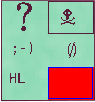
\includegraphics[width=95pt]{FIGS/Saisie/geometry.png}
\end{center}
\label{FIG:button1}
\end{figure}

The corresponding actions are:
\begin{itemize}
\item ;-) validate a point;
\item (/) unvalidate a point;
\item ? :
\item skull and bones: don't use the closest point (the point is displayed in red)
\item HL :
\item empty box: escape menu (do nothing)
\end{itemize}


\subsubsection{Info menu}

This menu can be shown with Shift + left-clic:

\begin{figure}[H]
\begin{center}
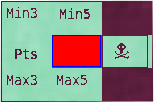
\includegraphics[width=154pt]{FIGS/Saisie/info.png}
\end{center}
\label{FIG:info}
\end{figure}

The corresponding actions are:
\begin{itemize}
\item Pts: select or add a name for this point
\item Min3:
\item Min5:
\item Max3:
\item Max5:
\item skull and bones: delete the point in all images (needs a confirmation)
\item empty box: escape menu (do nothing)
\end{itemize}

\subsubsection{Contextual menu}

This menu can be shown with Shift + right-clic:

\begin{figure}[H]
\begin{center}
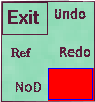
\includegraphics[width=95pt]{FIGS/Saisie/contextual.png}
\end{center}
\label{FIG:contextual}
\end{figure}

The corresponding actions are:

\begin{itemize}
\item Exit: quit the interface, saving {\tt Xml} files
\item Undo: undo last action
\item Redo: redo last action in history
\item Ref:
\item NoD/Ret: display or not the points names
\item empty box: escape menu (do nothing)
\end{itemize}

\subsubsection{Zoom menu}

This menu can be shown with Ctrl + right-clic:

\begin{figure}[H]
\begin{center}
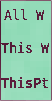
\includegraphics[width=52pt]{FIGS/Saisie/zoom.png}
\end{center}
\label{FIG:zoom}
\end{figure}

The three corresponding actions are:

\begin{itemize}
\item {\tt All W}: full zoom in all windows, and show images where points have not been measured yet;
\item {\tt This W}: zoom only in the window where the menu has been displayed;
\item {\tt This Point}: zoom on the nearest point in all windows where the point is visible
\end{itemize}


 %  -  -  -  -  -  -  -  -  -  -  -  -  -
\subsection{For bascule with {\tt SaisieBasc}}

\label{SaisieBasc}
 %  -  -  -  -  -  -  -  -  -  -  -  -  -
\subsection{For initial GCP  with {\tt SaisieAppuisInit}}
\label{SaisieAppuisInit}
 %  -  -  -  -  -  -  -  -  -  -  -  -  -

This section describes {\tt SaisieAppuisInit} the graphic interface to input 2D and 3D coordinates of ground control points.

For example with the Saint-Michel de Cuxa data set \ref{Cuxa:DataSet}:

\begin{verbatim}
SaisieAppuisInit  "Abbey-IMG_(021[12]|023[3456]).jpg"  All-Rel  NamePointInit.txt  MesureInit.xml
\end{verbatim}

When running this command, the interface shows data set's first images, where one can point GCPs:

\begin{figure}[H]
\begin{center}
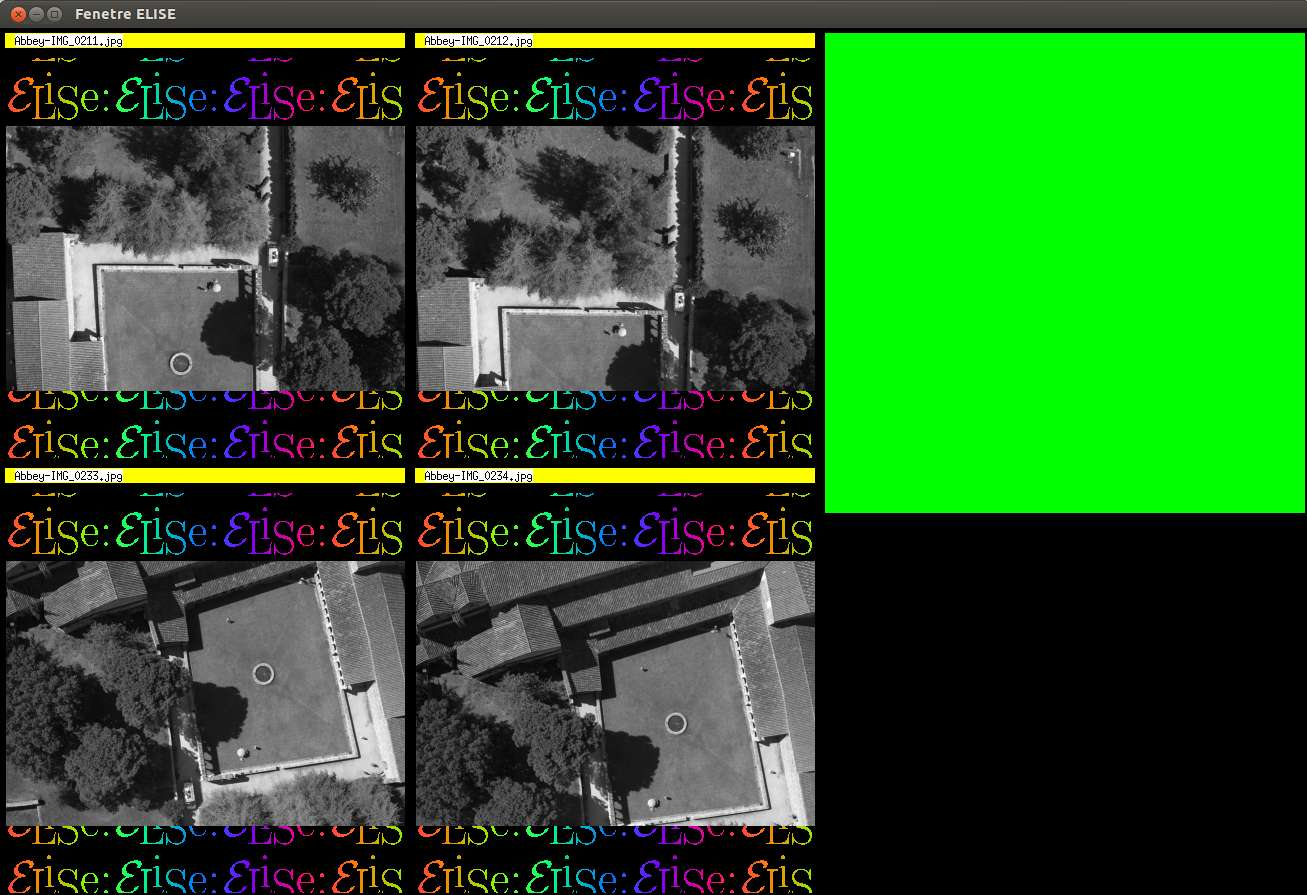
\includegraphics[width=150mm]{FIGS/Saisie/interface.jpg}
\end{center}
\caption{SaisieAppuis interface for ground control point selection}
\label{FIG:SaisieAppuis:interface}
\end{figure}

The general process for inputing ground control points is:
\begin{itemize}
\item Input a point in an image (Left-clic)
\item Select its name, 
\item Input the same point in the other images: move the yellow point and validate it with (right-clic + ;-) )
\item Iterate on each point you want to add (at each iteration, it can be usefull after having pointed the point in one image to zoom on this point in all the images,
this can be done by (Ctrl + right-clic + {\tt This Point})
\end{itemize}

When exiting the interface, two {\tt Xml} files are stored, with respectively 2D and 3D coordinates of input points.
Note that if for some reason some points are missing, you can re-run the same command, and continue the input job.
Points that have already been stored will be displayed, and the same process can be followed.

\subsection{For fast predictive entering GCP with {\tt SaisieAppuisPredic}}

When enough points have been selected, interface can give a prediction for each new input:

\begin{figure}[H]
\begin{center}
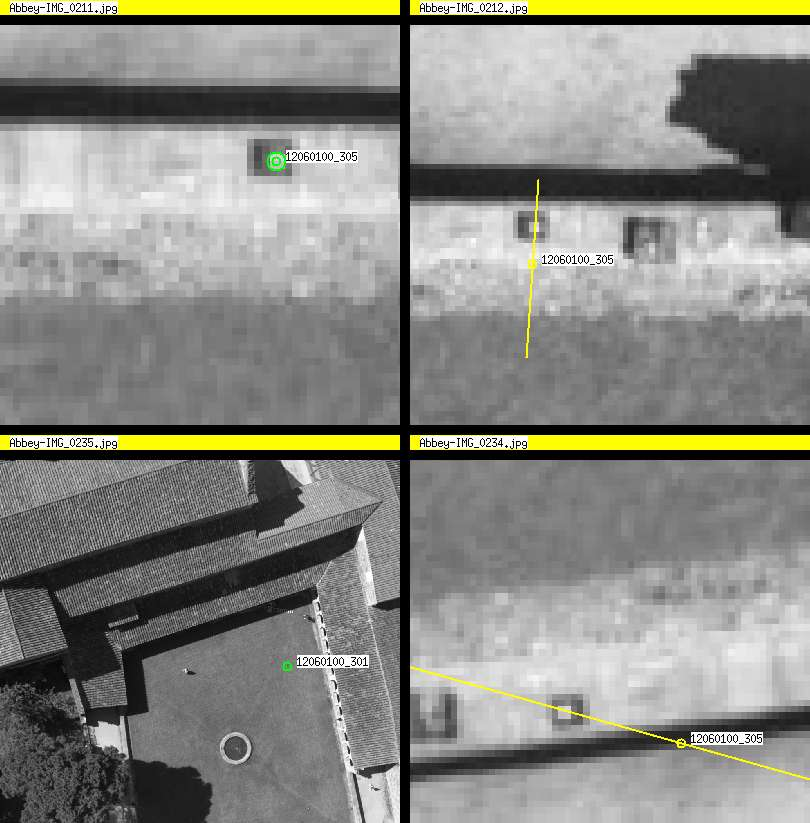
\includegraphics[width=120mm]{FIGS/Saisie/prediction.jpg}
\end{center}
\caption{Prediction help for adding new point}
\label{FIG:SaisieAppuis:prediction}
\end{figure}

%=======================================

\section{Visualize Tie-points with {\tt SEL}}

An old and uggly tool, but it can help. To visualize tie points computed with
{\tt Tapioca} :

\begin{verbatim}
SEL  ./ Face2-IMGP5331.JPG Face2-IMGP5333.JPG KH=NB
\end{verbatim}

For creating a few set of tie points and save in XML format :

\begin{verbatim}
SEL  ./ Face2-IMGP5331.JPG Face2-IMGP5333.JPG KH=S
\end{verbatim}



